

% Chapter Introduction
The researcher followed different methods and 
steps to conduct this study. The data gathering
procedures, experimental design, methods and steps 
and the statistical treatment of data are also 
included in this chapter.

% Research Design 
\section{Research Design}
The research design that is used in this study is 
is \emph{Single Group Design} which is a superset 
of \emph{Experimental Research Design}.

\section{Locale and Population of the Study}
The training of the various CNN Models and evaluation happened 
at a Google Colaboratory Session online. This was done because, 
a Google Colaboratory Session provides access to Graphical Processing 
Units (GPU) which massively speeds up the process of training the CNN Models.

\section{Data Gathering Instrument}
Data is the most important part of any type of Machine Learning Research. 
Since this research focuses on the feasibility of using a trained 
Convolutional Neural Network embedded in Smartphone Application to diagnose 
various plant diseases from an image of plant leaves, a plethora of 
healthy and infected plant leaf images were required to conduct this study. 

The researcher is in debt for the following datasets which were made publicly 
available. 

\begin{enumerate}
    \item \textbf{Plant Village Dataset}  \newline 
        - The PlantVillage dataset consists of $54303$ healthy and unhealthy leaf 
         images divided into $38$ categories by species and disease. 
    
         \begin{figure}[H]
            \centering 
            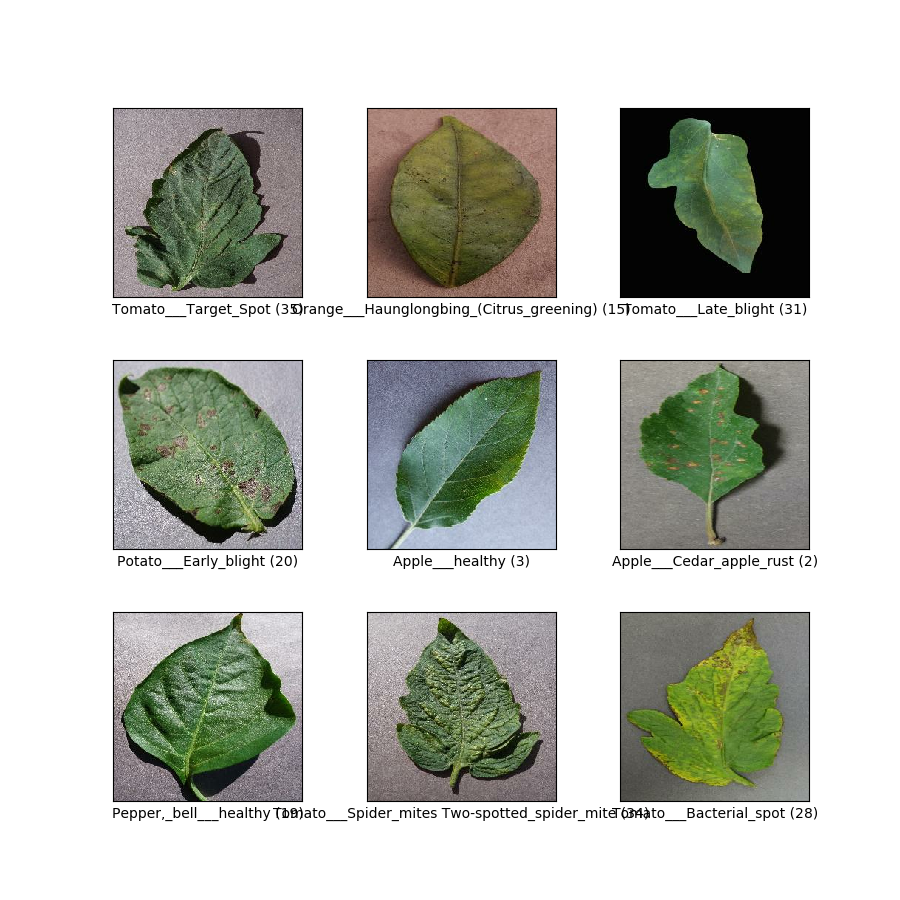
\includegraphics[scale=0.45]{plant-village-examples.png}
            \caption{Example of images in the Plant Village Dataset}
         \end{figure}


    \item \textbf{Citrus Dataset} \newline 
        - The dataset contains $759$ images of healthy and unhealthy images for both Citrus fruits and
         leaves collectively. Each image contains $256 \times 256$ dimensions with $72$ dpi resolution.  \\ 

         \begin{figure}[H]
            \centering 
            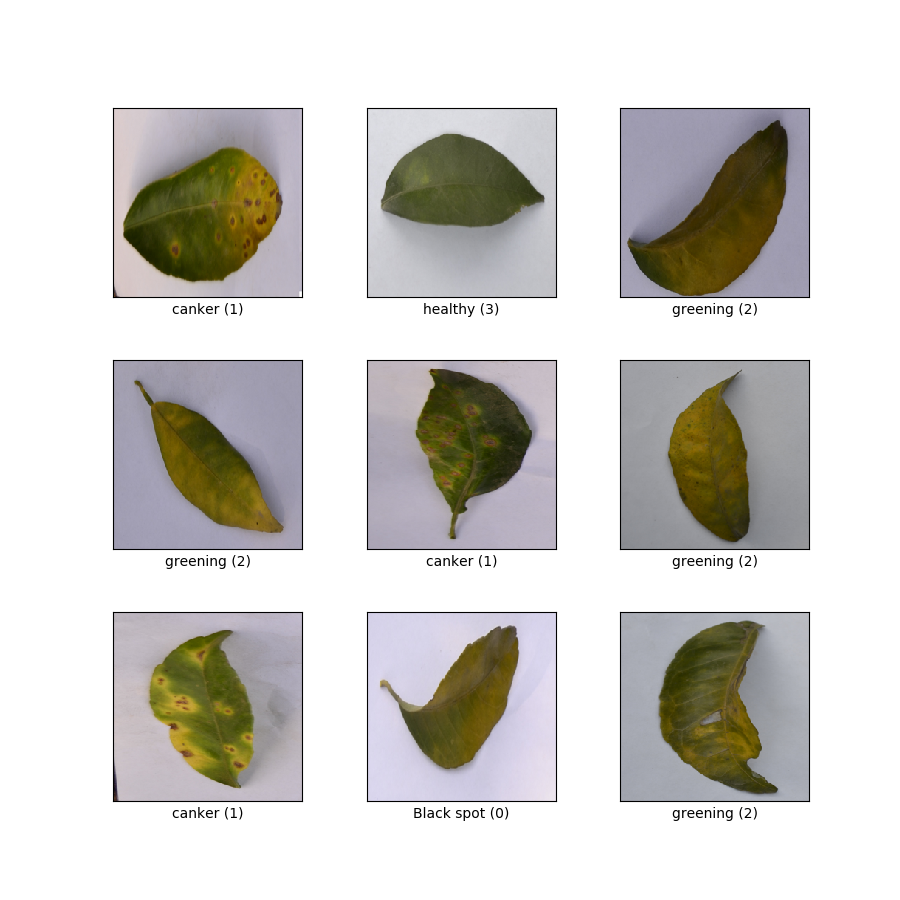
\includegraphics[scale=0.45]{citrus-leaves-examples.png}
            \caption{Example of images in the Citrus Leaves Dataset}
         \end{figure}

    % ! Temporary
    % \item \textbf{Field Images of Maize Annotated with Disease Symptoms} \\
    %     - This dataset consists of $18,222$ images annotated with 
    %     $105,705$ Northern Leaf Blight lesions.

\end{enumerate}

\section{Data Gathering Procedure}
In gathering the data required to conduct the study, the 
researcher downloaded the datasets from the following links.

\begin{itemize}
    \item https://data.mendeley.com/datasets/tywbtsjrjv/1
    \item https://data.mendeley.com/datasets/3f83gxmv57/2
\end{itemize}


\section{Statistical Treatment}

\subsection{Preprocessing of the Data}
After downloading the datasets through their official links, 
the datasets were then aggregated to a \emph{Google Colaboratory} 
session and were split into three sections, \emph{Training}, \emph{Validation} and 
\emph{Testing}, in a ratio of $ 60\% $, $ 20\% $, $ 20\% $ respectively. \\

The training dataset is used for training the various CNN Models while the Validation dataset 
gives an unbias representation of the accuracy of the model during the training process. Lastly, 
The testing dataset is used to gauge the accuracy of the model in detecting various plant diseases.
This was done to prevent the models from overfitting, and improve 
the accuracy of each model in classifying new data. 

\subsection{Training the Models}
To improve the overall accuracy and reduce the size 
of each models, the researcher opted to use a pre-trained model. 
A pretrained model is a type of model that was trained on a large 
dataset typical using a huge amount of computing power and time 
required to train. 

By introducing new layers on top of the pretrained model, the final 
CNN model will take less time to train and have improved accuracy in
classifying plant diseases.


\subsection{Testing the Models}
The ``F1 Score'' and ``Accuracy'' were the metrics
used to gauge the effectiveness of the model. 

\[ 
 \text{F1 Score} \: = \: \frac{2}{\frac{1}{\text{Precision}} \: + \: 
\frac{1}{\text{Recall}}} 
\]

\[
      \text{Accuracy} \: = \: \frac{\text{Precision} \: + \: 
      \text{Recall}}{\text{Total Number of Test Images}}
\]

